\documentclass[a4paper]{article}

\usepackage{cmap}
\usepackage[T2A]{fontenc}
\usepackage[english, russian]{babel}
\usepackage[utf8]{inputenc}
\usepackage[left=2cm,right=1.5cm,top=2cm,bottom=2cm]{geometry}
\usepackage{amsmath}
\usepackage{amssymb}
\usepackage{etoolbox}
\usepackage{amsthm}
\usepackage{booktabs}
\usepackage{graphicx}
\usepackage{tikz}
\usepackage{indentfirst}

\graphicspath{{./angem/}}

\newcommand{\Z}{\mathbb{Z}}
\newcommand{\N}{\mathbb{N}}
\newcommand{\R}{\mathbb{R}}
\newcommand{\Q}{\mathbb{Q}}
\newcommand{\B}{\mathfrak{B}}
\newcommand{\Bo}{\mathring{B}}
\renewcommand{\phi}{\varphi}
\renewcommand{\epsilon}{\varepsilon}
\renewcommand{\emptyset}{\varnothing}
\newcommand{\lra}{\Leftrightarrow}
\newcommand{\xn}{\{x_n\}_{n = 1}^{\infty}}
\renewcommand{\div}{\mid}
\newcommand{\ndiv}{\nmid}
\newcommand{\om}{\bar{\bar{o}}}
\newcommand\tab[1][.5cm]{\hspace*{#1}}

\newcommand{\lims}{\lim\limits_{n\to \infty}}
\renewcommand{\liminf}{\lim\limits_{x\to \infty}}
\newcommand{\liminfp}{\lim\limits_{x\to +\infty}}
\newcommand{\liminfm}{\lim\limits_{x\to -\infty}}
\newcommand{\lima}{\lim\limits_{x\to a}}
\newcommand{\limo}{\lim\limits_{x\to 0}}

\newcommand{\nl}{\newline}

\newcounter{concount}

\theoremstyle{plain}
\newtheorem{theorem}{Теорема}[section]
\newtheorem{corollary}{Следствие}[theorem]
\newtheorem{statement}{Утверждение}[section]

\theoremstyle{definition}
\newtheorem{definition}{Определение}[section]
\newtheorem{example}{Пример}[section]

\theoremstyle{remark}
\newtheorem{remark}{Замечание}[section]

\usepackage{titlesec}
\titleformat{\section}{\LARGE \bfseries}{\thesection}{1em}{}
\titleformat{\subsection}{\Large\bfseries}{\thesubsection}{1em}{}
\titleformat{\subsubsection}{\large\bfseries}{\thesubsubsection}{1em}{}

\usepackage{hyperref}
\usepackage{xcolor}
\definecolor{linkcolor}{HTML}{225ae2}
\definecolor{urlcolor}{HTML}{225ae2}
\hypersetup{
    pdfstartview=FitH, 
    linkcolor=linkcolor,
    urlcolor=urlcolor,
    colorlinks=true
}

\usetikzlibrary{calc}
\righthyphenmin=2 % разрешает перенос с двумя буквами на новой строке


%--------------------------------------------------------------------------
%--------------------------------------------------------------------------
%--------------------------------------------------------------------------
\title{Методичка по проективной геометрии}
%\author{Цыбулин Егор}
\date{\today}

\begin{document}
\maketitle
%\tableofcontents
\section{Проективная плоскость}
(Сипачёва) Одна из возможных моделей проективной плоскости - связки прямых и плоскостей в трёхмерном аффинном (или точечно-евклидовом) пространстве.
\begin{definition}[Комбаров]
    \textit{Проективная плоскость} P - произвольное множество, элементы которого называются \textit{точками}, и набор его подмножеств, именуемых \textit{прямыми} вместе с отношением инцидентности, если при этом выполняются аксиомы П1-П4. \nl
    П1. Любые две различные точки плоскости инцидентны одной и только одной прямой. \nl
    П2. Любые две различные прямые плоскости инцидентны одной и только одной точке. \nl
    П3. Существуют три точки, не инцидентные одной прямой. \nl
    П4. Каждая прямая инцидентна по меньшей мере трём точкам.
\end{definition}

\begin{definition}[Комбаров]
    Две проективные плоскости $P_1$ и $P_2$ называются \textit{изоморфными}, если существует биекция $f: P_1 \to P_2$, которая переводит точки в точки, прямые в прямые и сохраняет отношение инцидентности.
\end{definition}

(Сипачёва) Изоморфизмы между евклидовыми аффинными плоскостями тоже можно определить как биекции, сохраняющие структуры этих плоскостей: отображение одной евклидовой плоскости в другую является изоморфизмом тогда и только тогда, когда оно сохраняет расстояния между точками (и взаимно однозначно переводит прямые в прямые, но это можно не добавлять, так как эти условия выполнены автоматически, если сохраняются расстояния) - это мы доказали раньше; отображение одной аффинной плоскости в другую является изоморфизмом тогда и только тогда, когда оно взаимно однозначно и переводит прямые в прямые - это доказывается в курсе линейной алгебры.

В отличие от евклидовой и аффинной плоскостей, проективная плоскость определяется аксиомами неоднозначно: существуют неизоморфные проективные плоскости. Две проективные плоскости (точнее, две разные можели одной и той же проективной плоскости) мы уже построили и доказали, что они изоморфны. Ешё одну можно описать так:


\subsection{Плоскость Фано}
\noindent Точки - $A, \ B, \ C, \ D, \ E, \ F, \ G$ \nl
Прямые - $\{A, B\}, \ \{B, C\}, \ \{C, A\}, \ \{A, D\}, \ \{B, E\}, \ \{C, F\}, \ \{D, E, F\}$ \nl
Все аксиомы выполнены. Это минимальная модель проективной плоскости. \nl
\[ \begin{tikzpicture}[scale=0.8]

    % Координаты вершин треугольника
    \coordinate (A) at (0,0);
    \coordinate (B) at (4,0);
    \coordinate (C) at (60:3); % координата C задается в полярных координатах
    
    % Рисуем стороны треугольника
    \draw (A) node[left] {$A$} -- (B) node[right] {$B$} -- (C) node[above] {$C$} -- cycle;
    
    % Медиана к стороне AB
    \coordinate (M) at ($(A)!0.5!(B)$); % середина отрезка AB
    \draw[dashed] (C) -- (M);
    \node[below] at (M) {$D$}; % Название точки D
    
    % Медиана к стороне BC
    \coordinate (N) at ($(B)!0.5!(C)$); % середина отрезка BC
    \draw[dashed] (A) -- (N);
    \node[above] at (N) {$E$}; % Название точки E
    
    % Медиана к стороне AC
    \coordinate (P) at ($(A)!0.5!(C)$); % середина отрезка AC
    \draw[dashed] (B) -- (P);
    \node[below] at (P) {$F$}; % Название точки F
    
    % Точка пересечения медиан
    \coordinate (G) at (intersection of A--N and B--P); % точка пересечения двух медиан
    \node[circle,fill,inner sep=1pt,label={below right:$G$}] at (G) {};
    
\end{tikzpicture} \]
    
\begin{remark}
    Проективная плоскость не может содержать меньше семи точек.
\end{remark}

\begin{definition}[Сипачёва]
    \textit{Связка с центром О} - множество всех прямых и плоскостей трёхмерного пространства, проходящих через данную точку $O$. Прямые связки называются \textit{точками}, а плоскости - \textit{прямыми} проективной плоскости.
\end{definition}


\section{Перспективное соответствие}
(Сипачёва) Возьмём в аффинном пространстве какую-нибудь плоскость $\pi$, не проходящую через центр связки $O$. Через каждую точку $M$ плоскости $\pi$ проходит единственная прямая $OM$ связки (точка проективной плоскости), и через каждую прямую $l$ на плоскости $\pi$ проходит единственная плоскость связки (обозначим её $Ol$) (это прямая проективной плоскости).

Обратно, каждой прямой связки (если только она не параллельна $\pi$) соответствует единственная точка плоскости $\pi$, через которую она проходит. Каждой плоскости связки (не параллельной $\pi$) соответствует прямая на $\pi$.

Получилось почти биективное соответствие между точками (прямыми) проективной плоскости и точками (прямыми) на аффинной плоскости $\pi$. Чтобы сделать его совсем биективным, надо что-то поставить в соответствие прямым и плоскостям связки, которые параллельны $\pi$. Для этого плоскость $\pi$ придётся пополнить.


\section{Пополненная плоскость}
(Сипачёва) К каждой прямой $l \subset \pi$ добавим одну бесконечно удалённую точку. Эта точка будет соответствовать прямой связки, параллельной прямой $l$. Таким образом, ко всем прямым из несобственного пучка всех прямых, параллельных прямой $l$, будет добавлена одна и та же бесконечно удалённая точка. Её можно отождествить с самим несобственным пучком прямых на $\pi$, параллельных прямой $l$.

\begin{definition}
    \textit{Пополненная плоскость $\overline{\pi}$} - плоскость $\pi$ вместе с добавленными бесконечно удалёнными точками. \nl 
    \textit{Несобственные точки} - добавленные (бесконечно удалённые) точки. \nl 
    \textit{Несобственная прямая (бесконечно удалённая прямая)} - множество всех несобственных точек. \nl
    \textit{Собственные прямые пополненной плоскости $\overline{\pi}$} - прямые $l \subset \pi$ вместе с добавленными точками. \nl
    \textit{Собственные точки плоскости $\pi$} - точки плоскости $\pi$. Несобственная прямая соответствует плоскости связки, параллельной плоскости $\pi$.
\end{definition}

(Комбаров) Для данной прямой $l$ обычной плоскости $\pi$ обозначим через $[l]$ несобственный пучок прямых, параллельных прямой $l$.
Этот пучок $[l]$ назовём \textit{несобственной точкой} плоскости $\pi$.
Остальные её точки будем называть \textit{собственными}.
Добавим к плоскости $\pi$. все её несобственные точки и обозначим это новое множество через $\overline{\pi}$. Эти прямые обозначаются теми же символами $l$. Несобственная точка $[l]$ называется \textit{несобственной точкой прямой $l$}.
Множество $\overline{\pi} \ \pi$ всех несобственных точек называется \textit{несобственной прямой} расширенной плоскости $\overline{\pi}$.
Множество $\overline{\pi}$ с выделенными в нём собственными и несобственными прямыми называется \textit{пополненной плоскостью}.
Несобственные точки пополненной плоскости называются также \textit{бесконечно удалёнными}, несобственная прямая - \textit{бесконечно удалённой} прямой.
Напомним, что выражения "точка инцидентна прямой" и "прямая инцидентна точке" означают, что данная точка принадлежит данной прямой.

Пополненную плоскость моожно воспринимать и как множество всех пучков на плоскости как собственных, так и несобственных.
Если мы поставим в соответствие каждому собственному пучку прямых на плоскости центр этого пучка, то мы получим взаимно однозначное соответствие между всеми точками плоскости и всеми собственными пучками.
Каждый несобственный пучок мы отождествляем с несобственной точкой.
Собственные прямые пополняются несобственными точками.
При этом множество всех несобственных пучков объявляется несобственной прямой.

Итак, на проективной плоскости всякие две различные прямые $l_1$ и $l_2$ пересекаются в одной точке: собственной, если прямые $l_1$ и $l_2$ на обычной плоскости не параллельны, и несобственной, если параллельны.
Если одна из двух прямых несобственная, то она пересекается со второй прямой в единственной несобственной точке последней.
Легко видеть, что на проективной плоскости (так же как и на обыкновенной) через всякие две различные точки $M$ и $N$ проходит ровно одна прямая.
Это очевидно, если обе точки собственные.
Если $M$ - собственная, а $N$ - несобственная, то прямая $MN$ проходит через точку $M$ и принадлежит несобственному пучку, соответствующему точке $N$.
Наконец, если обе точки несобственные, то прямая $MN$ - несобственная прямая проективной плоскости.


\section{Однородные координаты}
(Сипачёва) Пусть в трёхмерном (аффинном) пространстве задана связка с центром $O$.
Возьмём какой-нибудь репер $Oe_1e_2e_3$ (с началом в $O$). Для каждой прямой $l$ из связки (точки проективной плоскости) координаты $(x_1, x_2, x_3)$ любого её направляющего вектора пропорциональны координатам любого другого её направляющего вектора.
Получается отношение эквивалентности между ненулевыми тройками координат: \[(x_1, x_2, x_3) \sim (y_1, y_2, y_3) \Leftrightarrow \exists \lambda (\neq 0) \in \R: \ (y_1, y_2, y_3) = (\lambda x_1, \lambda x_2, \lambda x_3). \]

Класс эквивалентности всех ненулевых троек координат, пропорциональных данной тройке $(x_1, x_2, x_3)$ (т.е. множество троек координат всех направляющих векторов прямой $l$) называется \textit{однородными координатами прямой $l$} в репере $Oe_1e_2e_3$ и обозначается $(x_1:x_2:x_3)$. Ясно, что однородные координаты любой прямой однозначно определяются любой тройкой координат из класса троек, представляющего собой эти однородные координаты, поэтому запись $(x_1:x_2:x_3)$ удобна и однозначно определяет однородные координаты; двоеточия говорят о том, что она определена с точностью до пропорциональности, т.е. 
\[ (x_1:x_2:x_3) =  (\lambda x_1, \lambda x_2, \lambda x_3), \ \forall \lambda \neq 0.\]

\textit{Однородные координаты точки} проективной плоскости (связки), которая является прямой $l$ связки, - это однородные координаты прямой $l$. Тем самым каждой точке проективной плоскости мы поставили во взаимно однозначное соответствие класс (множество) пропорциональных друг другу ненулевых троек чисел.

Каждая плоскость $\lambda$ (это прямая проективной плоскости) из связки задаётся уравнением вида 
\[ a_1x_1 + a_2x_2 + a_3x_3 = 0. \]
Тройки коэффициентов $\{a_1,a_2,a_3\}$ в разных уравнениях, задающих одну и ту же плоскость $\lambda$, пропорциональны друг другу.

\begin{definition}
    Класс всех (ненулевых пропорциональных друг другу) троек коэффициентов $\{a_1,a_2,a_3\}$ уравнений, задающих плоскость $\lambda$ в репере $Oe_1e_2e_3$, называется \textit{однородными координатами плоскости} $\lambda$ в репере $Oe_1e_2e_3$ и обозначается $\{a_1:a_2:a_3\}$.

    \textit{Однородные координаты прямой} проективной плоскости (т.е. плоскости в связке) - это однородные координаты соответствующей плоскости в связке.
\end{definition}

Таким образом, каждой прямой проективной плоскости мы тоже поставили во взаимно однозначное соответствие класс пропорциональных друг другу ненулевых троек чисел.

Точка проективной плоскости с однородными координатами $(x_1:x_2:x_3)$ \textit{инцидентна} прямой с однородными координатами $\{a_1:a_2:a_3\}$ тогда и только тогда, когда $a_1x_1 + a_2x_2 + a_3x_3 = 0$. Таким образом, в отношении инцидентности точки и прямые равноправны.

\begin{remark}
    Точки и прямые проективной плоскости равноправны всегда, не только в модели связки: легко показать, что аксиомы П1-П4 равносильны тем же аксиомам, в которых слова "точка"\ и "прямая"\ поменяны местами. Единственное, что отличает точку от прямой - это то, что прямая является множеством точек. Однако с тем же успехом можно объявить точку множеством всех инцидентных ей прямых.
\end{remark}


\section{Арифметическая модель проективной плоскости}
(Сипачёва) Рассмотрим два (совершенно идентичных) множества всех классов ненулевых пропорциональных друг другу троек чисел. Назовём классы троек из первого множества точками и будем записывать их в виде $(x_1:x_2:x_3)$, а классы из второго множества назовём прямыми и будем записывать их в виде $\{a_1:a_2:a_3\}$. 
Скажем, что точка $(x_1:x_2:x_3)$ и прямая $\{a_1:a_2:a_3\}$ инцидентны друг другу, если \[ a_1x_1 + a_2x_2 + a_3x_3 = 0. \]
Получилась почти проективная плоскость - все аксиомы выполнены, и есть лишь одна беда: прямые не являются множествами точек. Однако каждая прямая однозначно определяется множеством точек, которые ей инцидентны. Поэтому окончательное определение таково:

\begin{definition}
    \textit{Точки} - классы ненулевых троек чисел, пропорциональных друг другу, обозначаются $(x_1:x_2:x_3)$.
    \textit{Прямая} - множество всех точек (классов троек), удовлетворяющих одному и тому же уравнению вида \[ a_1x_1 + a_2x_2 + a_3x_3 = 0, \ a_1^2 + a_2^2 + a_3^2 \neq 0. \]
\end{definition}

Каждая прямая однозначно определяется ненулевой тройкой чисел, пропорциональной тройке $a_1, a_2, a_3$, т.е. классом ненулевых троек, пропорциональных $a_1, a_2, a_3$ (обозначается $\{a_1:a_2:a_3\}$), и наоборот - любой такой класс $\{a_1:a_2:a_3\}$ однозначно задаёт прямую. Таким образом, в рассуждениях прямые тоже можно отождествлять с тройками чисел, только надо помнить, что они другого сорта (однако если поменять местами роли прямых и точек, то ничего не изменится).

Получившаяся проективная плоскость называется \textit{арифметической моделью проективной плоскости}.

\begin{statement}
    Арифметическая модель проективной плоскости изоморфна и пополненной плоскости, и связке.
\end{statement}
\begin{proof}
    Изоморфизм между проективной плоскостью-связкой и арифметической моделью строится очевидным образом с помощью однородных координат. Изоморфизм между пополненной плоскостью и арифметической моделью получается как композиция изоморфизмов между пополненной плоскостью и связкой и между связкой и арифметической моделью.
\end{proof}

В дальнейшем под проективной плоскостью мы будем иметь в виду одну (любую) из этих изоморфных моделей.


\section{Принцип двойственности}
(Сипачёва) Неоднократно отмечавшееся выше равноправие точек и прямых проективной плоскости формулируется в виде принципа так:

\begin{theorem}[Принцип двойственности]
    Утверждение, касающееся точек и прямых проективной плоскости и отношения инцидентности между ними, верно тогда и только тогда, когда верно двойственное утверждение, которое получается из данного заменой слова "прямая"\ на "точка"\ и наоборот.
\end{theorem}

(Комбаров) В самом деле, числовое равенство \[ a_1x_1 + a_2x_2 + a_3x_3 = 0, \] выражающее условие инцидентности точки $(x_1:x_2:x_3)$ и прямой $\{a_1:a_2:a_3\}$, не зависит от того, какую из троек мы заключаем в круглые, а какую - в фигурные скобки. Принцип двойственности иллюстрирует равноправие точек и прямых на проективной плоскости, представленной рассматриваемыми моделями.

Рассмотрим пример двойственных утверждений. Две точки инцидентны одной и только одной прямой. Двойственное утверждение: две прямые инцидентны одной и только одной точке. Иными словами, аксиомы П1 и П2 являются двойственными утверждениями.


\section{Проективные системы координат}
\begin{definition}[Комбаров]
    Два репера $Oe_1e_2e_3$ и $Oe'_1e'_2e'_3$ с общим началом $O$ называются \textit{эквивалентными}, если существует такое число $\lambda$, что \[e'_i = \lambda e_i, \ i = 1,2,3.\]
\end{definition}

Следующее утверждение необходимо для последующего определения проективных координат.

\begin{statement}
    Реперы $Oe_1e_2e_3$ и $Oe'_1e'_2e'_3$ эквивалентны тогда и только тогда, когда каждая прямая связки $O$ имеет одни и те же однородные координаты в этих реперах.
\end{statement}
\begin{proof}
    В книге А.П. Комбарова, Ю.В. Садовничего "Аналитическая геометрия".
\end{proof}

\begin{definition}
    \textit{Проективной системой координат в связке $O$} называется класс эквивалентных между собой аффинных реперов (или, что то же самое, аффинных систем координат) с началом $O$.
\end{definition}

Проективная система координат в связке $O$ однозначно определяется упорядоченной четвёркой прямых $X_1, X_2, X_3, E$ связки, таких что никакие три прямые не лежат в одной плоскости. Такая четвёрка прямых (точек проективной плоскости) называется \textit{фундаментальной четвёркой}. Прямые $X_1, X_2, X_3$ называются координатными, а $E$ - единичной.

\begin{definition}
    Тройки однородных координат произвольной прямой связки $O$ в аффинном репере $Oe_1e_2e_3$, или, что то же самое, в любом аффинном репере, эквивалентном реперу $Oe_1e_2e_3$, называются \textit{тройками проективных координат} этой прямой в проективной системе $X_1, X_2, X_3, E$.
\end{definition}

\[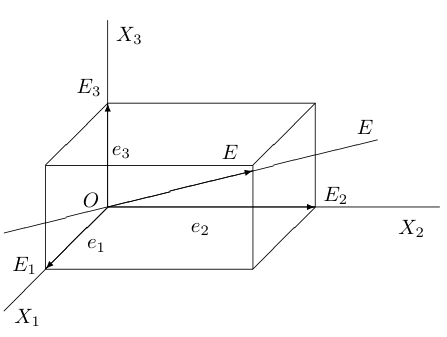
\includegraphics{1.png}\]

В частности, прямые $X_1, X_2, X_3, E$ имеют в этой системе координат следующие координаты:
\[ X_1 = (1:0:0), \ X_2 = (0:1:0), \ X_3 = (0:0:1), \ E = (1:1:1). \]


\subsection{Переход от одной проективной системы координат к другой}
Пусть на проективной плоскости P заданы две проективные системы координат - исходная, "старая"\ $X_1X_2X_3E$ и "новая"\ система $X'_1X'_2X'_3E'$. Выберем какой-нибудь параллелепипед, соответствующий "новой"\ системе координат, и запишем координаты векторов $e'_1, e'_2, e'_3$, совпадающих со сторонами параллелепипеда, в "старой"\ системе координат $Oe_1e_2e_3$. То есть, "новая"\ система задана какими-то тройками проективных координат относительно "старой"\ системы:
\[ \begin{cases}
    X'_1 = (c_{11} : c_{21} : c_{31}), \\
    X'_2 = (c_{12} : c_{22} : c_{32}), \\
    X'_3 = (c_{13} : c_{23} : c_{33}), \\
    X'_1 = (\epsilon_1 : \epsilon_2 : \epsilon_3).
\end{cases} \]
Надо найти формулы преобразования координат, выражающие координаты $x_1, x_2, x_3$ любой точки $m$ относительно "старой"\ системы координат через координаты $x'_1, x'_2, x'_3$ той же точки в "новой"\ системе координат. Заметим, что, поскольку был выбран конкретный параллелепипед, тройки координат точек $X'_1, X'_2, X'_3, E'$ выбраны согласованными, т.е. подчинены условию
\[ (c_{11} : c_{21} : c_{31}) + (c_{12} : c_{22} : c_{32}) + (c_{13} : c_{23} : c_{33}) = (\epsilon_1 : \epsilon_2 : \epsilon_3). \]
Тогда, возвращаясь к связке $O$ и предполагая, что ("старая") проективная система $X_1X_2X_3E$ порождается аффинным репером $Oe_1e_2e_3$, видим, что векторы
\[ e'_1 = \{c_{11}, c_{21}, c_{31}\}, \ e'_2 = \{c_{12}, c_{22}, c_{32}\}, \ e'_3 = \{c_{13}, c_{23}, c_{33}\}, \]
заданные координатами в базисе $e_1, e_2, e_3$, линейно независимы, поскольку прямые $X_1, X_2, X_3$ не лежат в одной плоскости. Заметим, что матрица
\[C = \begin{pmatrix} c_{11}&c_{12}&c_{13} \\ c_{21}&c_{22}&c_{23} \\ c_{31}&c_{32}&c_{33} \end{pmatrix}\]
является матрицой перехода от базиса $e_1, e_2, e_3$ к базису $e'_1, e'_2, e'_3$, то есть
\[ (e'_1, e'_2, e'_3) = (e_1, e_2, e_3) \cdot C. \]
Далее, каждая тройка $x_1, x_2, x_3$ проективных координат в системе $X_1X_2X_3E$ произвольной прямой $m$ есть тройка координат в репере $Oe_1e_2e_3$ некоторого направляющего вектора $a$ этой прямой.
Аналогичным образом тройка координат $x'_1, x'_2, x'_3$ прямой $m$ в системе $X'_1X'_2X'_3E'$ есть тройка координат в репере $Oe'_1e'_2e'_3$ какого-то направляющего вектора $a' = \lambda a$ той же прямой $m$.
Поэтому из формул преобразования аффинных координат получаем
\[ \lambda \begin{pmatrix}
    x_1 \\ x_2 \\ x_3
\end{pmatrix} = 
\begin{pmatrix} c_{11}&c_{12}&c_{13} \\ c_{21}&c_{22}&c_{23} \\ c_{31}&c_{32}&c_{33} \end{pmatrix}
\begin{pmatrix}
    x'_1 \\ x'_2 \\ x'_3
\end{pmatrix}. \]
Здесь $\lambda$ - множитель, принимающий все отличные от нуля значения. Это и есть формула перехода от проективной системы $X_1X_2X_3E$ к проективной системе $X'_1X'_2X'_3E'$.


\section{Линии второго порядка на проективной плоскости}
(Сипачёва) Будем рассматривать проективную плоскость как пополненную плоскость $\overline{\pi}$.
При этом $\pi$ задаётся уравнением $x_3 = 1$ в некотором аффинном репере $Oe_1e_2e_3$ в трёхмерном пространстве, а $\overline{\pi}$ получается из $\pi$ добавлением бесконечно удалённых точек.
Реперу $Oe_1e_2e_3$ соответствует репер $Oe_1e_2$ на $\pi$.
Будем рассматривать однородные координаты точек $\overline{\pi}$, которые получаются с использованием этого же репера.

Линия второго порядка на $\pi$ задаётся уравнением
\[ \begin{pmatrix} x&y&1 \end{pmatrix} A \begin{pmatrix} x \\ y \\ 1 \end{pmatrix} = 0, \
A = \begin{pmatrix}
    a_{11} & a_{12} & a_{13} \\ a_{21} & a_{22} & a_{23} \\ a_{31} & a_{32} & a_{33}
\end{pmatrix}
\]

Перейдём к однородным координатам
\[ x = \frac{x_1}{x_3}, \ y = \frac{x_2}{x_3}: \]
\begin{equation} \label{1}
    \begin{pmatrix} x_1 & x_2 & x_3 \end{pmatrix} A \begin{pmatrix} x_1 \\ x_2 \\ x_3 \end{pmatrix} = 0,
\end{equation}
т.е.
\[ a_{11} x_1^2 + a_{22} x_2^2 + a_{33} x_3^2 + 2a_{12} x_1 x_2 + 2a_{13} x_1 x_3 + 2a_{23} x_2 x_3 = 0. \]

\begin{definition}
    Линией второго порядка на проективной плоскости называется множество точек проективной плоскости, проективные координаты которых удовлетворяют уравнению вида \eqref{1}, где $A \neq 0$, в некоторой проективной системе координат.
\end{definition}

На пополненной плоскости уравнению \eqref{1} удовлетворяют, во-первых, все собственные точки, однородные координаты которых удовлетворяют уравнению \eqref{1} (т.е. обычные координаты в репере $Oe_1e_2$ удовлетворяют уравнению $ \begin{pmatrix} x&y&1 \end{pmatrix} A \begin{pmatrix} x \\ y \\ 1 \end{pmatrix} = 0$).

\begin{remark}
    Заметим, что это не обязательно линия второго порядка на $\pi$, так как ненулевая матрица $A$ может иметь вид $\begin{pmatrix} 0&0&a_{13} \\ 0&0&a_{23} \\ a_{13}&a_{23}&a_{33} \end{pmatrix}$, а тогда это прямая вида $2a_{13}x + 2a_{23}y + a_{33} = 0$.
\end{remark}

Несобственные точки (с однородными координатами $(x_1 : x_2 : 0)$), удовлетворяющие уравнению \eqref{1}, т.е. такие, что $a_{11}x_1^2 + 2a_{12} x_1 x_2 + a_{22} x_2^2 = 0$.
Они отвечают асимптотическим направляениям линии второго порядка на $\pi$, заданной уравнением $ \begin{pmatrix} x&y&1 \end{pmatrix} A \begin{pmatrix} x \\ y \\ 1 \end{pmatrix} = 0$, если не все элементы $a_{11}, a_{12}, a_{22}$ матрицы $A$ равны $0$.
Если же они все равны $0$, то уравнению \eqref{1} удовлетворяют все несобственные точки пополненной плоскости $\overline{\pi}$, т.е. вся несобственная прямая.

Итак, всякая линия второго порядка на пополненной плоскости - это либо
\begin{itemize}
    \item линия второго порядка на $\pi$, пополненная асимптотическим направлением, либо
    \item пара пересекающихся прямых, одна из которых несобственная (когда $a_{11} = a_{12} = a_{22} = 0$ и $a^2_{12} + a^2_{23} \neq 0$), либо
    \item пара совпадающих несобственных прямых (когда $a_{11} = a_{12} = a_{13} = a_{22} = a_{23} = 0$, в этом случае $a_{33} \neq 0$, т.к. $A \neq 0$).
\end{itemize}

\begin{definition}
    Уравнения вида \eqref{1} линий второго порядка на проективной плоскости \textit{проективно эквивалентны}, если одно из них можно превратить в другое проективной заменой координат.
\end{definition}

У нас есть соответствующие друг другу реперы $Oe_1e_2e_3$ в пространстве и $Oe_1e_2$ на $\pi$. Мы знаем, что если $a^2_{11} + a^2_{12} + a^2_{22} \neq 0$ (1 случай), то аффинной заменой координат матрицу $A$ можено привести к виду $\begin{pmatrix} a'_{11}&0&0 \\ 0&a'_{22}&0 \\ 0&0&a'_{33} \end{pmatrix}$ (не парабола) или $\begin{pmatrix} 0&0&a'_{13} \\ 0&a'_{22}&0 \\ a'_{13}&0&0 \end{pmatrix}$ (парабола), где $a'_{11}, a'_{22}, a'_{33} = \pm 1 \ \text{или} \ 0; \ a'_{22} = a'_{13} = 1$.

Рассмотрим возможные разновидности пересечения нашей проективной линии с $\pi$.
\begin{enumerate}
    \item \textit{Эллипс}: $x^2 + y^2 = 1$. В однородных координатах: $x^2_1 + x^2_2 - x^2_3 = 0$.
    \item \textit{Гипербола}: $x^2 - y^2 = 1$. В однородных координатах: $x^2_1 - x^2_2 - x^2_3 = 0 \Leftrightarrow -x^2_1 + x^2_2 + x^2_3 = 0$. \nl 
    Проективная замена координат $\begin{cases} \lambda x_1 = x'_3, \\ \lambda x_2 = x'_1, \\ \lambda x_3 = x'_2 \end{cases}$
    приводит это уравнение к виду: $x_1^{'2} + x_2^{'2} - x_3^{'2} = 0$.
    \item \textit{Парабола}: $y^2 - 2x = 0$. В однородных координатах: $x_2^2 - 2x_1 x_3 = 0$. 
    Проективная замена $\begin{cases}
    \lambda x_1 = x'_2, \\
    \lambda x_2 = \frac{x'_2 + x'_1}{\sqrt{2}}, \\
    \lambda x_3 = \frac{x'_3 - x'_1}{\sqrt{2}}
    \end{cases}$
    приводит это уравнение к виду $x_1^{'2} + x_2^{'2} - x_3^{'2} = 0$.


Вывод: Уравнение линий второго порядка на проективной плоскости, собственные точки которой образуют эллипс, гиперболу или параболу, проективно эквивалентны.

\begin{definition}
    Линия второго порядка на проективной плоскости, которая в некоторой проективной системе координат описывается уравнением $x_1^{2} + x_2^{2} - x_3^{2} = 0$, называется \textit{овалом}.
\end{definition}

    \item \textit{Мнимый эллипс}: $x^2 + y^2 + 1 = 0$. В однородных координатах: $x_1^2 + x_2^2 + x_3^2 = 0$. Эта линия называется \textit{мнимым овалом}. Это пустое множество.
    \item \textit{Пара пересекающихся прямых}: $x^2 - y^2 = 0$. В однородных координатах: $x_1^2-x_2^2 = 0$. Это и в проективной плоскости пара пересекающихся прямых.
    \item \textit{Пара мнимых пересекающихся прямых (точка)}: $x^2 + y^2 = 0$. В однородных координатах: $x_1^2 + x_2^2 = 0$. Это, по-прежнему, точка.
    \item \textit{Пара совпадающих прямых}: $y^2 = 0$, т.е. $x_2^2 = 0$. Это уравнение проективно эквивалентно $x_1^2 = 0$.
    \item \textit{Параллельные прямые}: $y^2 - 1 = 0$. В однородных координатах: $x_2^2 - x_3^2 = 0$. Проективно эквивалентно уравнению пары пересекающихся прямых.
    \item \textit{Мнимые параллельные прямые}: $y^2 + 1 = 0$, т.е. $x_2^2 + x_3^2 = 0$. Проективно эквивалентно уравнению пары мнимых пересекающихся прямых.
\end{enumerate}

Итак, существуют 5 классов проективной эквивалентности уравнений линий второго порядка на проективной плоскости:
\begin{enumerate}
    \item $x_1^2 + x_2^2 - x_3^2 = 0$ - овал;
    \item $x_1^2 + x_2^2 + x_3^2 = 0$ - мнимый овал;
    \item $x_1^2 - x_2^2 = 0$ - пара пересекающихся прямых;
    \item $x_1^2 + x_2^2 = 0$ - пара мнимых пересекающихся прямых (точка);
    \item $x_1^2 = 0$ - пара совпадающих прмяых.
\end{enumerate}

\begin{statement}
    Уравнения 1.-5. попарно НЕ проективно эквивалентны. Следует помнить, что с точки зрения проективной плоскости собственные и несобственные прямые на пополненной плоскости совершенно равноправны, т.к. их уравнения можно преобразовать друг в друга проективной заменой координат.
\end{statement}


\section{Проективные преобразования}
(Сипачёва)
\begin{definition}
    Отображение $f: P \to P$ проективной плоскости P в себя называется проективным преобразованием, если существуют две проективные системы координат $X_1X_2X_3E$ и $\tilde{X_1}\tilde{X_2}\tilde{X_3}\tilde{E}$ такие, что $\forall M \in P$ точка $f(M)$ имеет во второй системе координат те же координаты, что $M$ имела в первой.
\end{definition}
\begin{remark}
    Очевидно, это биекция.
\end{remark}

Ситуация совершенно аналогична случаю линейных преобразований. Если $C$ - матрица перехода от $X_1X_2X_3E$ к $\tilde{X_1}\tilde{X_2}\tilde{X_3}\tilde{E}$, т.е. от аффинного репера (какого-нибудь из них), определяющего проективный репер $X_1X_2X_3E$, к аффинному реперу, определяющему $\tilde{X_1}\tilde{X_2}\tilde{X_3}\tilde{E}$, то координаты $(x_1 : x_2 : x_3)$ точки $M$ относительно первого репера выражаются через её координаты $(\tilde{x_1} : \tilde{x_2} : \tilde{x_3})$ относительно второго так:
\[ \begin{pmatrix}
    \lambda x_1 \\
    \lambda x_2 \\
    \lambda x_3
\end{pmatrix} = C
\begin{pmatrix}
    \tilde{x_1} \\
    \tilde{x_2} \\
    \tilde{x_3}
\end{pmatrix}.
\]
Пусть $(x'_1 : x'_2 : x'_3)$ - координаты в $X_1X_2X_3E$  точки $f(M)$, где $M\simeq (x_1 : x_2 : x_3)$. Тогда
\[ \lambda \begin{pmatrix}
    x_1 \\
    x_2 \\
    x_3
\end{pmatrix} = C
\begin{pmatrix}
    \tilde{x_1} \\
    \tilde{x_2} \\
    \tilde{x_3}
\end{pmatrix}.
\]
Матрица $C$ называется \textit{матрицей проективного преобразования} $f$.

\begin{statement}
    Пусть $l$ - прямая с координатами ${a_1 : a_2 : a_3}$ на проективной плоскости. Тогда $f(l)$ - прямая с координатами $\{a_1 : a_2 : a_3\}C^{-1}$.
\end{statement}

\begin{definition}
    Линии второго порядка на проективной плоскости \textit{проективно эквиваленты}, если одну из них можно перевести в другую проективным преобразованием.
\end{definition}

\begin{remark}
    В отличие от евклидова и аффинного случаев, линии второго порядка на проективной плоскости проективно эквивалентны тогда и только тогда, когда их уравнения проективно эквивалентны.
\end{remark}

\section{Теорема Дезарга}
\begin{theorem}
    Если прямые, проходящие через соответственные вершины треугольников $A_1B_1C_1$ и $A_2B_2C_2$, пересекаются в одной точке, то точки пересечения соответственных сторон лежат на одной прямой.
\end{theorem}
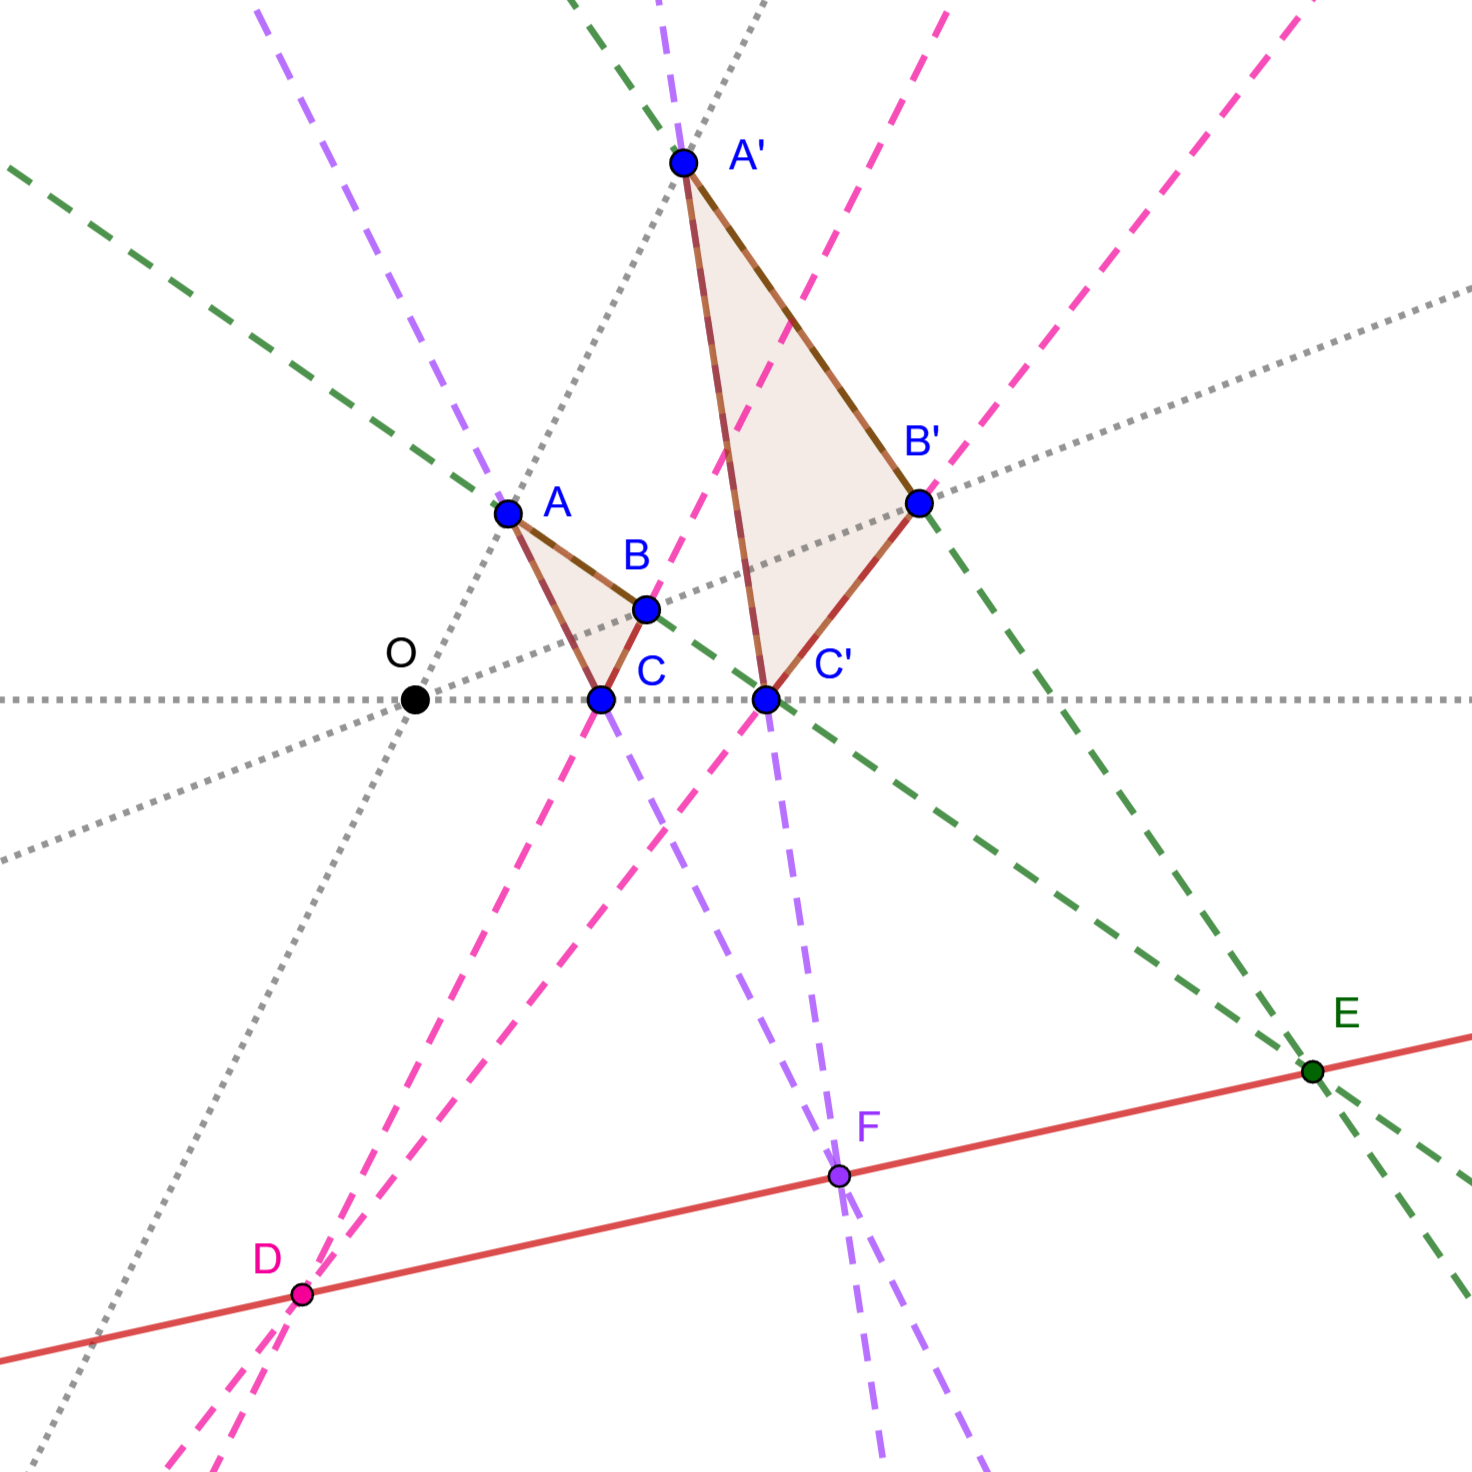
\includegraphics{теорема Дезарга.png}

\end{document}